\section{Equal-Loudness-Level Contours}
\label{Equal-loudness-level-contours}
Igennem de efterfølgende afsnit vil der blive givet en kort introduktion til tre af de mest betydningsfulde undersøgelser inden for \textit{Loudness}, hvor den sidste undersøgelse, \textcite{STD:ISO226}, danner grundlag for resten af rapporten. 
%
\subsection{Fletcher og Munson}
\label{Fletcher-Munson}
%
Den første undersøgelse af hvordan mennesket perciperer rene toner ved forskellige frekvenser i det hørbareområde, som går fra 20Hz til 20000Hz, blev foretaget af \textcite{PDF:FletcherMunson}. Sammenhængen mellem perceptionen af \textit{Loudness} for rene toner og frekvens blev målt på 11 forsøgspersoner, som alle udførte forsøget med høretelefoner på, \parencite[s. 86]{PDF:FletcherMunson}. Formålet var at måle et \textit{Loudness Level} ved at justere lydtryksniveauet af en referencetone, en ren tone på 1000Hz, så den lød lige så høj som den tone, den blev sammenlignet med, \parencite[s. 84]{PDF:FletcherMunson}. De toner som referencen blev sammenlignet med var i frekvensområdet 62Hz til 16000Hz, \parencite[s. 88]{PDF:FletcherMunson}. Resultatet af denne undersøgelse blev det første sæt \textit{Loudness-Level Contours}, og illustreres på \autoref{fig:FletcherMunson}.
%
\begin{figure}[H]
	\centering
	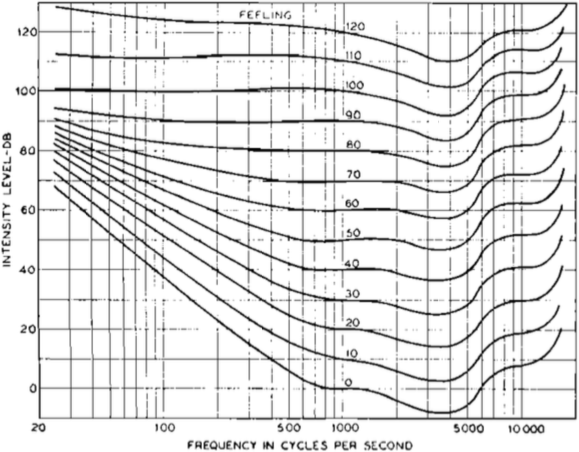
\includegraphics[resolution=300,width=\textwidth]{FletcherMunson}
	\caption{\textit{Loudness-Level Contours}, som blev udarbejdet af \textcite[s. 91]{PDF:FletcherMunson}. Hvor x-aksen angives som \textit{Frequency in cycles per second}, hvilket er den tidligere engelske betegnelse for frekvens i hertz, og y-aksen angiver lydtryksniveauer i dB.  Kurverne er angivet i værdier fra 0 til 120, med en stepsize på 10, og disse værdier svarer hver især til en specifik phon-kurve.}
	\label{fig:FletcherMunson}
\end{figure}
\noindent
%
Baseret på \autoref{fig:FletcherMunson} tyder det på at frekvenser under 1000Hz skal have et højere lydtryksniveau for at blive perciperet på samme måde, som referencetonen. Dog med forbehold for at ved høje lydtryksniveauer, over 80dB, udglattes kurverne, hvilket indikerer at lave frekvenser tilnærmelsesvist skal have det samme lydtryksniveau som referencen. Dykket ved samtlige kurver på \autoref{fig:FletcherMunson} skyldes at mennesker er mest sensitive overfor frekvenser i området fra 2000Hz til 5000Hz, \parencite{WEB:HowLoudIsTooLoud}.
\blankline
Ud fra den beskrevne eksperimentelle metode fremgår det at forsøget blev udført i et lydtæt rum, hvor forsøgspersonerne skulle vurdere om referencetonen var højere eller lavere end den tone der blev testet for, \parencite[s. 104]{PDF:FletcherMunson}. Derudover fremgår det, at der under forsøget var mere end én forsøgsperson inde i det lydtætte rum, \parencite[s. 104]{PDF:FletcherMunson}. Hver af de to forsøgspersoner skulle angive deres respons ved at trykke på nogle knapper, med henblik på at forsøgspersonernes respons således ikke ville påvirke hinanden, men det er uvist hvorvidt det har haft indflydelse på forsøgspersonernes respons at der var endnu en forsøgsperson i rummet. Dertil er undersøgelsen foretaget af \textcite{PDF:FletcherMunson} begrænset til kun at undersøge hvordan lyd perciperes igennem høretelefoner og er ikke foretaget i et frit felt, men i et lydtæt rum hvor høretelefonerne er kalibreret i forhold til rummet, så det giver effekten af et tilnærmelsesvist frit felt.\\
Grundet en stigende interesse på området blev der senere udført flere undersøgelser vedrørende mennesket perception af lyd, hvoraf en af dem er særligt nævneværdig; \textcite{PDF:RobinsonDadson}, som blev den første standard for \textit{Equal-Loudness Contours} og var den gyldige ISO226 indtil 2003. 
%
\newpage
\noindent
%
\subsection{Robinson og Dadson}
\label{Robinson-Dadson}
Undersøgelsen foretaget af \textcite[s. 166]{PDF:RobinsonDadson} er den første version af standarden ISO226, og beskriver forholdet mellem \textit{Equal-Loudness} og rene toner i et frit felt. Ligesom ved den førnævnte undersøgelse blev en ren referencetone på 1000Hz valgt til forsøget. Referencen blev sammenlignet med andre rene toner indenfor frekvensområdet fra 25Hz til 15000Hz og op til 130dB, \parencite[s. 167]{PDF:RobinsonDadson}. Undersøgelsen bygger på data indsamlet fra to grupper, hvor den ene gruppe bestod af 90 forsøgspersoner med begge køn ligeligt repræsenteret og et aldersspænd fra 16år til 63år. De deltog i omkring 30 forsøg. Den anden gruppe bestod af 30 forsøgspersoner, 17 mænd og 13 kvinder med en gennemsnitsalder på 30år, som deltog i over 100 forsøg, \parencite[s. 167]{PDF:RobinsonDadson}. Alle forsøgspersonerne der deltog i undersøgelsen blev forundersøgt for eventuelle høreskader og andre øresygdomme.\\
Forsøgspersonerne blev bedt om at vurdere hvilken af de to afspillede rene toner der var højest. Referencetonen var konstant 1000Hz men varierede i lydtryksniveau og den anden tone forblev konstant både i frekvens og lydtryksniveau, \parencite[s. 168]{PDF:RobinsonDadson}. Resultatet fra undersøgelsen fremgår af \autoref{fig:RobinsonDadson-Curves}.
%
\begin{figure}[H]
	\centering
	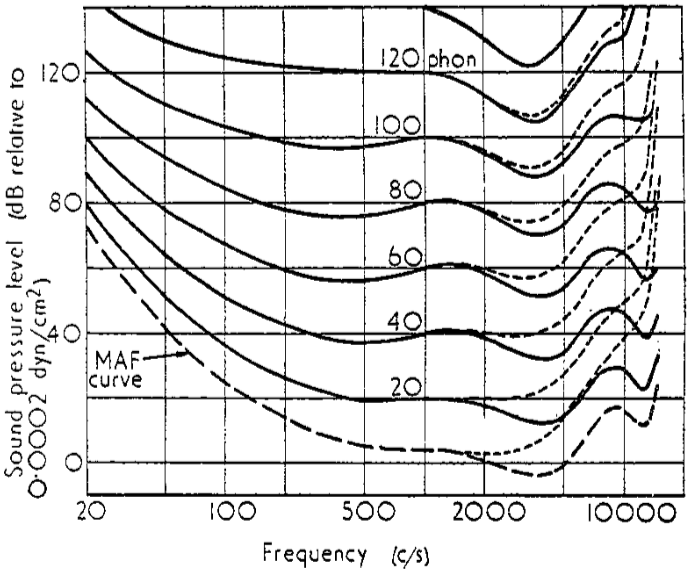
\includegraphics[resolution=300,width=\textwidth]{RobinsonDadson-Curves}
	\caption{\textit{Equal-Loudness Contours}, som blev udarbejdet af \textcite[s. 171]{PDF:RobinsonDadson}. X-aksen angiver frekvens i c/s, hvilket svarer til hertz og y-aksen angiver lydtryksniveauet. Kurverne er aldersopdelt, så de stiplede kurver repræsenterer aldersgruppen centreret omkring 60årige og kontinuerte kurver repræsenterer aldersgruppen centreret om 20årige forsøgspersoner.}
	\label{fig:RobinsonDadson-Curves}
\end{figure}
\noindent
%
\textcite[s. 171]{PDF:RobinsonDadson} fandt at ved frekvenser fra 25Hz til og med 1000Hz var der ingen aldersmæssig forskel, men fra 1000Hz og op forekom der en forskel, hvilket ligeledes fremgår af \autoref{fig:RobinsonDadson-Curves}.
\blankline
Ifølge \textcite[s. 918]{PDF:EqualLoudnessForPureTones} er der de senere år opstået ny interesse for \textit{Equal-Loudness-Level Contours} hvilket har resulteret i flere videnskabelige undersøgelser. Fælles for disse undersøgelser er, at de afviger fra resultaterne fundet af \textcite[s. 171]{PDF:RobinsonDadson}, særligt ved omkring 800Hz og ned hvor der måles et højere \textit{Equal-Loudness} niveau, \parencite[s. 918]{PDF:EqualLoudnessForPureTones}. Den store mængde af nye undersøgelser har været med til at danne grundlag for den nye, aktuelle standard; \textcite{STD:ISO226}.
%
\subsection{ISO226}
\label{ISO226}
%
I modsætning til både \textcite{PDF:FletcherMunson} og \textcite{PDF:RobinsonDadson} bygger \textcite[s. 9]{STD:ISO226} på 12 uafhængige videnskabelige undersøgelser, som alle lever op til følgende seks kriterier, fremsat i \textcite[s. 1]{STD:ISO226};
\blankline
\begin{alpherate}
  \item the sound field in the absence of the listener consists of a free progressive plane wave;
  \item the source of sound is directly in front of the listener;
  \item the sound signals are pure tones;
  \item the sound pressure level is measured at the position where the centre of the listener's head would be, but in the absence of the listener;
  \item listening is binaural;
  \item the listeners are otologically normal persons in the age range from 18 years to 25 years inclusive.
\end{alpherate}
\blankline
\noindent
%
Ydermere er frekvensområdet for de rene toner defineret til at være mellem 20Hz og 12500Hz, hvor frekvenserne vælges efter step af en tredjedel oktav. Resultaterne fra de 12 undersøgelser, som udgør \textcite{STD:ISO226}, er illustreret på \autoref{fig:EqualLoudnessContoursGraph} og går under navnet: \textit{Normal Equal-Loudness-Level Contours}.
%
\newpage
\noindent 
%
\begin{figure}[H]
	\centering
	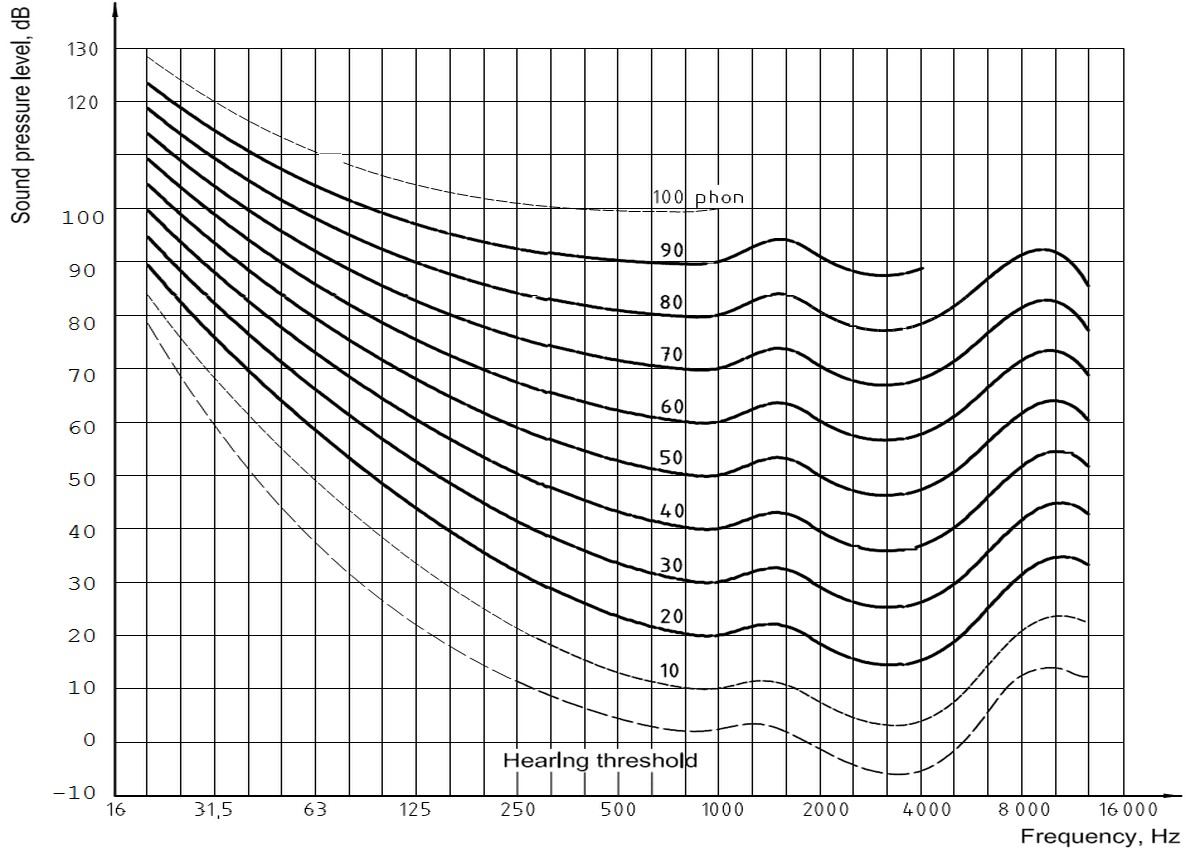
\includegraphics[resolution=300,width=\textwidth]{EqualLoudnessContoursGraph}
	\caption{\textit{Normal-Equal-Loudness-Level Contours} for rene toner fremsat i \textcite[s. 5]{STD:ISO226}. Hvor de stiplede kurver indikerer at der ikke forefindes tilstrækkeligt med eksperimentel data, x-aksen angiver frekvens i hertz og y-aksen angiver lydtryksniveau i dB.}
	\label{fig:EqualLoudnessContoursGraph}
\end{figure}
\noindent
%
\autoref{fig:EqualLoudnessContoursGraph} illustrerer det lydtryksniveau en given ren tone skal spilles ved for at lyde lige så høj som referencetonen på 1000Hz ved forskellige phon-kurver. Ved 80phon-kurven vil en ren tone på 125Hz eksempelvis skulle afspilles ved et lydtryksniveau på 90dB, for at lyde lige så høj som referencen på 1000Hz ved 80dB. Dette vil blive perciperet som en fordobling i lydtryksniveau, da mennesker generelt perciperer en stigning på 10dB som værende minimum en fordobling i lydtryksniveau, \parencite{PDF:Music175Loudness}.\\
Det fremgår således at perceptionen af rene toner både afhænger af frekvens og lydtryksniveau, hvor lavfrekvente toner vil blive perciperet, som om de afspilles ved et lavere lydtryksniveau, sammenlignet med højfrekvente toner ved det samme lydtryksniveau. Det vil derfor være nødvendigt at forstærke lavfrekvente toner for at de perciperes som værende lige så høje, som højfrekvente toner. Hvor meget de rene toner skal forstærkes, eller dæmpes, fremgår af \autoref{app:ISO226Raadata}.
\blankline
Som tidligere nævnt, anvendes en ren 1000Hz tone ved forskellige lydtryksniveauer som reference og enheden for disse lydtryksniveauer i referencepunktet er phon, som blev defineret i \fullref{Loudness}. Med den viden er det muligt at beregne hvilket lydtryksniveau en ren tone, ved en bestemt frekvens, skal afspilles ved for at blive perciperet lige så høj som referencen, ved en given phon-kurve. Dette gøres via følgende udtryk, som blev udledt i \textcite[s. 2]{STD:ISO226}:
\blankline
Hvor lydtryksniveauet $L_{P}$ for en ren tone med frekvensen $f$ er et \textit{Loudness Level} $L_{N}$, givet ved: 
%
\begin{equation} \label{eq:SPL_Fra_Loudness}
	 L_p=\left(\frac{10}{\alpha_f} * lg A_f\right) dB - L_U + 94dB		
\end{equation}
\noindent
%
Hvor $A_{f}$ gives ved:
%
\begin{equation} \label{eq:SPL_Fra_Loudness_Tilfoejelse}
	A_f = 4.47 * 10^{-3} * \left(10^{0.025*L_N} - 1.15\right) + \left[0.4*10^{\left(\frac{T_f + L_U}{10} - 9\right)}\right]^{\alpha_f}
\end{equation}
\noindent
%
Hvor:
\begin{itemize}
	\item[] $T_f$ er høretærsklen
	\item[] $\alpha_f$ er eksponenten for perception af \textit{Loudness}
	\item[] $L_U$ er størrelsen af den lineære overføringsfunktion normaliseret ved 1000Hz\\[5mm]
\end{itemize}
\noindent
%
Disse udtryk gør sig kun gældende fra 20phon til 90phon, med forbehold for at 90phon er begrænset til frekvenserne fra 20Hz til 4000Hz og 80phon er begrænset til frekvenserne fra 5000Hz til 12500Hz, \parencite[s. 2]{STD:ISO226}. Alt uden for denne afgrænsning fungerer udelukkende informativt.
\blankline
Baseret på de foregående afsnit kan det konkluderes at menneskets perception af rene toner ændres afhængigt af frekvens og lydtryksniveau; desto lavere frekvensen er, desto større lydtryksniveau skal der til for at tonen bliver perciperet lige så høj, som referencen. Ydermere er mennesket mest sensitiv overfor toner i frekvensområdet fra 2000Hz til 5000Hz, hvilket er årsagen til dykket på, blandt andet, \autoref{fig:EqualLoudnessContoursGraph}. 
%
\newpage
\noindent